\documentclass[10pt,a4paper,twocolumn]{article}
\newcommand{\runningtitle}{Baryon-antibaryon reconstruction at 50 MeV}
\newcommand{\paperfooter}{Revised research manuscript | 18 October 2026}
\usepackage[utf8]{inputenc}
\usepackage[T1]{fontenc}
\usepackage{lmodern}
\usepackage[margin=17mm,top=18mm,bottom=19mm,columnsep=6.5mm]{geometry}
\usepackage{amsmath,amssymb,array,booktabs,graphicx,xcolor,microtype}
\usepackage[authoryear,round]{natbib}
\usepackage{caption,stfloats,fancyhdr,balance}
\usepackage{multicol}
\usepackage[unicode,colorlinks=true,linkcolor=navy,citecolor=navy,urlcolor=navy]{hyperref}
\definecolor{navy}{HTML}{173B56}
\setlength{\parindent}{1em}
\setlength{\parskip}{1pt}
\raggedbottom
\clubpenalty=10000
\widowpenalty=10000
\setlength{\emergencystretch}{1.7em}
\setlength{\intextsep}{9pt}
\setlength{\textfloatsep}{11pt}
\setlength{\dbltextfloatsep}{11pt}
\setcounter{topnumber}{3}
\setcounter{dbltopnumber}{2}
\renewcommand{\topfraction}{.92}
\renewcommand{\dbltopfraction}{.95}
\renewcommand{\textfraction}{.08}
\renewcommand{\floatpagefraction}{.82}
\renewcommand{\dblfloatpagefraction}{.82}
\captionsetup{font=small,labelfont=bf,labelsep=period,skip=5pt}
\pagestyle{fancy}
\fancyhf{}
\fancyhead[L]{\footnotesize\color{navy}\runningtitle}
\fancyhead[R]{\footnotesize Andrés Germán García}
\fancyfoot[L]{\footnotesize\paperfooter}
\fancyfoot[R]{\footnotesize\thepage}
\setlength{\headheight}{13pt}
\renewcommand{\headrulewidth}{.35pt}
\newcommand{\fB}{f^{(s)}_{B\bar B}}
\newcommand{\sB}{s_{B+\bar B}}
\newcommand{\stot}{s_{\mathrm{tot}}}
\newcommand{\shad}{s_{\mathrm{had}}}
\newcommand{\sL}{s_{\mathrm{light}}}
\newcommand{\YB}{Y_{\Delta B}}
\newcommand{\doi}[1]{\href{https://doi.org/#1}{doi:#1}}
\newcommand{\fulltitle}[3]{%
\twocolumn[%
\begin{center}
{\fontsize{18}{20.5}\selectfont\bfseries\color{navy}#1\par}
\vspace{8pt}
{\normalsize Andrés Germán García\par}
{\small #2\par}
\vspace{7pt}
{\small #3\par}
\end{center}
\vspace{6pt}
\begin{minipage}{\textwidth}
\textbf{\abstractlabel.} \abstracttext
\vspace{6pt}\par
\textbf{\keywordslabel:} \keywordstext
\end{minipage}
\vspace{15pt}
]%
}


\newcommand{\abstractlabel}{Abstract}
\newcommand{\keywordslabel}{Keywords}
\newcommand{\abstracttext}{We reconstruct separate baryon and antibaryon equilibrium populations from fixed hadronic inventories, temperature, and a cosmological net-baryon-to-entropy constraint. An ideal hadron resonance gas is evaluated with PDG2014, PDG2020, and PDG2025 lists, retaining nominal masses and spin degeneracies. The baryon chemical potential is determined while $\mu_Q=\mu_S=0$. At 50 MeV, PDG2025 yields $2.7261\times10^{30}$ baryons and $2.7172\times10^{30}$ antibaryons per cm$^3$, with a net excess of $8.8765\times10^{27}$ cm$^{-3}$. There are 306.1147 antibaryons per unit of net excess, and nucleons and antinucleons contribute 95.2176\% of the total. The criterion $n_{\bar B}=n_B-n_{\bar B}$ occurs at 38.203739 MeV, which rounds to the published reference of 38.2 MeV. Varying only the input $\eta=(6.12\pm0.04)\times10^{-10}$ gives 38.192814--38.214598 MeV. Comoving normalization relates these populations to an explicit present volume, while a rank test shows that the residual alone cannot identify a unique pair population or history. All 24 numerical checks and five archived CSV outputs were reproduced; a further momentum-integral calculation checks aggregate densities and entropy at two states. The baseline leaves nonzero net charge and strangeness. It provides a reproducible equilibrium reference; chemical-neutrality controls and kinetic evolution belong to the companion extension. Numerical agreement does not determine total physical uncertainty.}
\newcommand{\keywordstext}{baryon abundance; annihilation; thermal equilibrium; rest mass; retrospective reconstruction; hadronic resonances.}
\hypersetup{pdftitle={Baryon-Antibaryon Reconstruction at 50 MeV: Rest Masses and Cosmological Abundances},pdfauthor={Andrés Germán García}}
\begin{document}
\fulltitle{Baryon-Antibaryon Reconstruction at 50 MeV:\\Rest Masses and Cosmological Abundances}{Independent Researcher, Mexico}{Original version: 9 October 2026 | Revised: 18 October 2026}
\section{Introduction}
Present baryon abundance retains information about the excess of matter over antimatter, but reconstructing the quantities that coexisted during annihilation requires establishing what additional information a thermal model supplies. Two inventories with the same difference between baryons and antibaryons can contain very different pair populations. The retrospective question must therefore distinguish the observed residual from the total population inferred at a specified temperature.

The literature provides concrete reference points for this comparison. \citet{Satarov2013} describe nearly equal baryon and antibaryon abundances above approximately 50 MeV and a rapid decrease in the antibaryon fraction as the plasma cools below that scale. \citet{Yang2022} investigate the 50--30 MeV window and report 38.2 MeV for the criterion $n_{\bar B}/(n_B-n_{\bar B})=1$. These reference points describe abundance evolution; 50 MeV is not a measurement of the first annihilation event, and the second criterion does not require antibaryons to have disappeared.

The hadron resonance gas (HRG) permits equilibrium populations to be calculated from the rest masses, spins, and charges of particle species. Thermal-FIST lists provide a documented inventory for this calculation \citep{Vovchenko2019,TFLists2026}. In this work, these tabulated properties constitute the signatures used to identify each particle species. No original spectral signals from the early epoch were analyzed. Present cosmological abundance was incorporated as an external constraint on net baryon number.

The objective was to test whether these properties, combined with present abundance and a temperature grounded in the literature, permit separate inference of early baryon and antibaryon populations, quantification of their relationship to the residual, and comparison with published results. Whether the present determines a unique historical reconstruction was also examined. The analysis focused on 50 MeV and the location of the published abundance crossing, retaining the HRG inventory masses and stating the conditions that enable the inference.

\section{Methods}
\subsection{Design, data, and inventory scope}
A mathematical reconstruction of equilibrium states was performed. A temperature of 50 MeV was adopted as an approximate literature reference, and points between 37 and 50 MeV were evaluated to locate the abundance crossing. Intermediate points were numerical evaluations without assignments to additional physical epochs. Natural units, $\hbar=c=k_B=1$, were used, with masses and temperatures in GeV.

The PDG2014, PDG2020, and PDG2025 lists were read from the Thermal-FIST repository, fixed at revision \texttt{4086191e9522} \citep{TFLists2026}. The supplement contains the full identifier, original files, license, and SHA-256 hashes. Nominal masses and spin degeneracies were retained; commented lines and entries with zero degeneracy were excluded. Each charge state was counted according to its entry, and antiparticles were included separately where applicable. All active baryonic entries had $|B_i|=1$.

\begin{table}[t]
\centering\small
\caption{Dimensions of the inventories used. Active species include antiparticles; $B+\bar B$ counts active baryonic entries.}
\label{tab:inventory}
\setlength{\tabcolsep}{4pt}
\begin{tabular}{lrrr}\toprule
List & Rows & Active species & $B+\bar B$\\\midrule
PDG2014 & 219 & 387 & 260\\
PDG2020 & 242 & 433 & 298\\
PDG2025 & 248 & 443 & 292\\
\bottomrule\end{tabular}
\end{table}

The lists cover the $u,d,s$ quark sector; no nuclei or lists from other quark sectors were added. An ideal HRG with fixed masses, zero resonance widths, and a common temperature was adopted. Excluded-volume corrections and reaction evolution were not incorporated. The conditions $\mu_Q=\mu_S=0$ were maintained, and $\mu_B$ was solved for. This simplification does not impose electric neutrality or zero net strangeness; lepton chemical potentials that would compensate the charge were not solved for either.

\subsection{Densities and entropy per particle species}
For each massive particle species, the number density was calculated as
\begin{equation}
n_i=\frac{g_i m_i^2T}{2\pi^2}
\sum_{k=1}^{K_{\max}}\frac{c_{i,k}}{k}
K_2(kx_i)e^{k\alpha_i},\label{eq:number}
\end{equation}
where $x_i=m_i/T$, $\alpha_i=\mu_i/T$, and $\mu_i=B_i\mu_B$. Here $g_i=2J_i+1$; $c_{i,k}=1$ for bosons and $c_{i,k}=(-1)^{k+1}$ for fermions. $K_\nu$ denotes the modified Bessel function of the second kind. These expressions implement Bose-Einstein and Fermi-Dirac distributions; they do not describe a statistical test on measurements.

Entropy was obtained using the same chemical potential:
\begin{align}
s_i&=\frac{g_i m_i^2T}{2\pi^2}
\sum_{k=1}^{K_{\max}}c_{i,k}e^{k\alpha_i}\bigg[
\frac{4K_2(kx_i)}{k^2}\nonumber\\
&\qquad+\frac{x_iK_1(kx_i)}{k}
-\frac{\alpha_iK_2(kx_i)}{k}\bigg].\label{eq:entropy}
\end{align}
The sums used 96 terms, with 192 terms for the convergence check. Mesons had $\mu_i=0$. Total entropy included hadrons, photons, electrons and positrons, muons and antimuons, and three flavors of neutrinos and antineutrinos:
\begin{equation}
s_{\rm tot}=s_{\rm had}+s_\gamma+s_{e^\pm}
+s_{\mu^\pm}+s_{\nu\bar\nu}.\label{eq:stotal}
\end{equation}
Photons, electrons, and neutrinos were treated as massless components, with combined degeneracies of 2, 4, and 6. The expression $s_{\rm rel}=(2\pi^2/45)gT^3$ was used, multiplied by $7/8$ for fermions. Muons were calculated as massive particles with $m_\mu=0.1056583755$ GeV and combined degeneracy 4 \citep{PDG2025}. Chemical potentials in the light sector were set to zero.

The quantities $n_\Sigma=n_B+n_{\bar B}$ and $\Delta n_B=n_B-n_{\bar B}$ were defined, together with $Y_i=n_i/s_{\rm tot}$. In physical units, the yield denominator is $s_{\rm tot}/k_B$, expressed in the same volume units as $n_i$. Natural-unit densities were converted to cm$^{-3}$ using $\hbar c=1.973269804\times10^{-14}$ GeV cm \citep{Robinson2025}. Temperature conversion used $k_B=8.617333262\times10^{-5}$ eV K$^{-1}$.

\subsection{Cosmological constraint and inverse solution}
The value $\eta=(6.12\pm0.04)\times10^{-10}$ was adopted as an external CMB input, compiled by \citet{Fields2025}. Adiabatic conservation of entropy and net baryon number gave
\begin{equation}
\frac{\Delta n_B(T,\alpha)}{s_{\rm tot}(T,\alpha)}
=Y_{\Delta B}^{\rm ref}=\frac{\eta}{7.04},
\quad\alpha=\frac{\mu_B}{T}.\label{eq:inverse}
\end{equation}
The factor 7.04 converts present abundance per photon to abundance per entropy under the standard approximation after $e^+e^-$ annihilation. The condition $s(T)/n_\gamma(T)=7.04$ was not imposed on the 50 MeV plasma.

To avoid loss of precision from subtracting nearly equal populations, $a_{i,k}=g_i m_i^2T c_{i,k}K_2(kx_i)/(2\pi^2k)$ was defined for entries with $B_i=+1$, and the following expressions were evaluated:
\begin{align}
n_\Sigma&=2\sum_{i,k}a_{i,k}\cosh(k\alpha),\nonumber\\
\Delta n_B&=2\sum_{i,k}a_{i,k}\sinh(k\alpha).\label{eq:stable}
\end{align}
Pair entropy was summed equivalently using hyperbolic functions. Equation~\eqref{eq:inverse} was solved using Brent's method over $0\leq\alpha\leq1$, with absolute tolerance $10^{-18}$ and relative tolerance $10^{-13}$. The populations were recovered as $n_B=(n_\Sigma+\Delta n_B)/2$ and $n_{\bar B}=(n_\Sigma-\Delta n_B)/2$.

To compare the same criterion as \citet{Yang2022}, the ratio was defined as
\begin{equation}
R(T)=\frac{n_{\bar B}}{\Delta n_B}
=\frac{Y_{\bar B}}{Y_{\Delta B}}.\label{eq:ratio}
\end{equation}
A second root calculation located $R(T_\times)=1$ within 37--40 MeV, with absolute tolerance $10^{-10}$ MeV and relative tolerance $10^{-13}$. This interval provided a numerical bracket for the crossing, rather than an initial temperature adjusted to produce agreement. The solution was repeated with the three catalogs and at the endpoints $\eta=6.08$ and $6.16\times10^{-10}$, varying only this input.

\subsection{Comparison with the present and uniqueness test}
With $T_{\gamma0}=2.7255\pm0.0006$ K, rounded from \citet{Fixsen2009}, the following quantities were calculated:
\begin{align}
n_{\gamma0}&=\frac{2\zeta(3)}{\pi^2}
\left(\frac{k_BT_{\gamma0}}{\hbar c}\right)^3,\nonumber\\
s_0/k_B&\simeq7.04n_{\gamma0},\qquad
n_{b0}=\eta n_{\gamma0}.\label{eq:present}
\end{align}
To compare quantities within the same comoving region, $s(T)V(T)=s_0V_0$ was used, and hence
\begin{equation}
N_i(T)=Y_i(T)(s_0/k_B)V_0.\label{eq:comoving}
\end{equation}
The value $V_0=1$ m$^3$ was chosen as an explicit normalization; the resulting numbers are mean quantities and may be fractional. No volume for the entire Universe was adopted.

The primordial composition equivalent at the present mean density was converted using $Y_p=0.245\pm0.003$ and $(D/H)_{\rm P}=(2.508\pm0.029)\times10^{-5}$ \citep{Fields2025}: $n_{H0}^{\rm prim}\simeq(1-Y_p)n_{b0}$, $n_{{}^4He,0}^{\rm prim}\simeq Y_p n_{b0}/4$, and $n_{D0}^{\rm prim}\simeq(D/H)_{\rm P}n_{H0}^{\rm prim}$. Corrections from trace nuclei to the H/He balance, binding corrections, stellar processing, and ionization were neglected. Uncertainties were propagated to first order assuming independent inputs; the outputs share inputs and are correlated.

Uniqueness was examined using the map $(Y_B,Y_{\bar B})\mapsto Y_B-Y_{\bar B}$. Its matrix $[1,-1]$ has rank one and null direction $(1,1)$. This property identifies the information missing from the residual without proposing additional kinetic histories.

\subsection{Verification and uncertainty treatment}
The 24 recorded checks compared 96 and 192 terms, verified closure of the cosmological constraint, and compared proton and neutron number densities, excess, and entropy with independent integrals at finite chemical potential. Catalog hashes were verified, and aggregate and particle-species results were exported. Tables and figures were generated directly from these files.

For the present revision, the original calculation was rerun and its five CSV outputs were compared byte for byte with the archived results. An additional Python program, importing no project functions, integrated the momentum distributions for the 443 active PDG2025 species and the specified light bath at 50 MeV and at the crossing. It shared the catalog, temperatures, and solved chemical potentials with the reference calculation, and compared the aggregate $n_B$, $n_{\bar B}$, $\Delta n_B$, and $s_{\rm tot}$. This checks a different numerical evaluation of the same state; it does not independently infer the chemical potential or supply new observational inputs.

No hypothesis tests, fits to new observations, or random simulations were performed. Variation among catalogs measures inventory sensitivity, and the interval obtained from $\eta$ propagates a single input; neither represents the total physical error of the HRG. Convergence errors assess the numerical implementation. No $p$ values or statistical significance for proximity to 38.2 MeV were calculated.

\section{Results}
\subsection{Populations reconstructed at 50 MeV}
The central cosmological input fixed $Y_{\Delta B}^{\rm ref}=8.69318\times10^{-11}$. With this same excess per entropy unit, the PDG2025 HRG at 50 MeV ($5.8023\times10^{11}$ K) yielded $n_B=2.7261\times10^{30}$ and $n_{\bar B}=2.7172\times10^{30}$ cm$^{-3}$. The sum was $5.4433\times10^{30}$ cm$^{-3}$ and the net excess was $8.8765\times10^{27}$ cm$^{-3}$ (Table~\ref{tab:states}). These four values are results of the inverse calculation; the net yield was the imposed external condition.

The ratio $R=306.1147$ means that approximately 306.1 antibaryons and 307.1 baryons coexisted per unit of net excess in this state. The ratio $n_{\bar B}/n_B=0.996744$ was obtained: approximately 99.6744 antibaryons per 100 baryons. The excess represented 0.163071\% of the sum. The solution required $\mu_B/T=0.00163071$, equivalent to $\mu_B=0.0815356$ MeV.

\begin{table*}[t]\centering\small
\caption{Reconstructed PDG2025 states at the central input $\eta$. Densities refer to physical volume at each temperature; $R=n_{\bar B}/\Delta n_B$.}
\label{tab:states}
\setlength{\tabcolsep}{6pt}
\begin{tabular}{rrrrrr}\toprule
$T$ (MeV) & $n_B$ (cm$^{-3}$) & $n_{\bar B}$ (cm$^{-3}$) & $\Delta n_B$ (cm$^{-3}$) & $R$ & $\mu_B/T$\\\midrule
50.0 & $2.7261\times10^{30}$ & $2.7172\times10^{30}$ & $8.8765\times10^{27}$ & 306.114688 & 0.001631\\
45.0 & $2.8323\times10^{29}$ & $2.7694\times10^{29}$ & $6.2899\times10^{27}$ & 44.028849 & 0.011229\\
40.0 & $1.9166\times10^{28}$ & $1.4894\times10^{28}$ & $4.2724\times10^{27}$ & 3.486095 & 0.126100\\
38.203739 & $7.3454\times10^{27}$ & $3.6727\times10^{27}$ & $3.6727\times10^{27}$ & 1.000000 & 0.346574\\
37.0 & $4.4167\times10^{27}$ & $1.1116\times10^{27}$ & $3.3051\times10^{27}$ & 0.336326 & 0.689799\\
\bottomrule\end{tabular}
\end{table*}


Protons, neutrons, and their antiparticles contributed 95.2176\% of the total baryonic population at 50 MeV; the other catalog baryons contributed 4.7824\%. Table~\ref{tab:nucleons50} identifies the nucleon contributions with their retained rest masses. The entropy fraction of the baryon-antibaryon sector was $s_{B+\bar B}/s_{\rm tot}=1.15182\times10^{-6}$; this entropy fraction differs from a fraction of particle number.

\begin{table}[t]\centering\small
\caption{Nucleons and their antiparticles at 50 MeV, PDG2025. Density is given in units of $10^{30}$ cm$^{-3}$.}
\label{tab:nucleons50}
\begin{tabular}{lrr}\toprule
Particle species & Mass (MeV) & Density\\\midrule
$p$ & 938.272 & 1.313384\\
$\bar p$ & 938.272 & 1.309107\\
$n$ & 939.565 & 1.282334\\
$\bar n$ & 939.565 & 1.278159\\
\bottomrule\end{tabular}
\end{table}


\subsection{Thermal sequence and abundance crossing}
As temperature decreased from 50 to 45 and 40 MeV, $R$ decreased from 306.1147 to 44.02885 and 3.486095. At the published temperature of 38.2 MeV, $R=0.997012$ was obtained; the independently calculated root was $T_\times=38.203739$ MeV (Figure~\ref{fig:cross}). The crossing rounds to 38.2 MeV at the precision reported by \citet{Yang2022}. The arithmetic difference, $+0.003739$ MeV, does not provide a statistical precision for the agreement.

At the PDG2025 root, $n_{\bar B}=\Delta n_B=3.6727\times10^{27}$ cm$^{-3}$ and $n_B=7.3454\times10^{27}$ cm$^{-3}$. By definition, $R=1$ implies $n_B=2n_{\bar B}$, $n_{\bar B}/n_B=1/2$, and an excess equal to one third of the sum. Antibaryons were still present at this reference point. The nucleon contribution reached 98.8254\%.

\begin{figure*}[t]
\centering
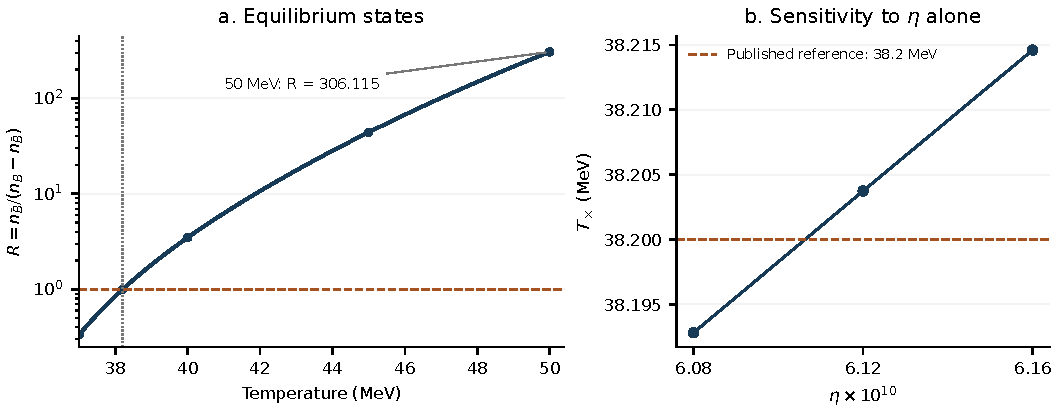
\includegraphics[width=.98\textwidth]{figures/final_cross_en.pdf}
\caption{Antibaryon-to-net-excess ratio for PDG2025. Left: sequence of equilibrium states between 37 and 50 MeV; points indicate this work's evaluations and the horizontal line indicates $R=1$. Right: crossing temperature obtained for the central value and endpoints of the input uncertainty in $\eta$; the line between points is a visual guide. The reference at 38.2 MeV is from Yang and Rafelski (2022); no unpublished uncertainty is assigned to it.}
\label{fig:cross}
\end{figure*}

The three inventories yielded nearby crossings (Table~\ref{tab:crosscatalogs}). Between PDG2014 and PDG2025, the numerical range was $0.000142$ MeV. Varying only $\eta$ within $(6.12\pm0.04)\times10^{-10}$ gave a PDG2025 crossing interval of 38.192814--38.214598 MeV and an $R(50)$ interval of 304.1237--308.1319. This input sensitivity exceeded both the difference from the rounded literature value and the range obtained with these three catalogs.

\begin{table}[t]\centering\small
\caption{Inventory sensitivity at the same cosmological input. Extra decimal places document the calculation, not its physical accuracy.}
\label{tab:crosscatalogs}
\begin{tabular}{lrr}\toprule
List & $T_\times$ (MeV) & $R(50\ {\rm MeV})$\\\midrule
PDG2014 & 38.203596 & 306.128980\\
PDG2020 & 38.203739 & 306.114776\\
PDG2025 & 38.203739 & 306.114688\\
\bottomrule\end{tabular}
\end{table}


\subsection{Quantities within the same comoving region}
The cosmological conversions gave $n_{\gamma0}=410.7268$ cm$^{-3}$ and $n_{b0}=(2.514\pm0.017)\times10^{-7}$ cm$^{-3}$, compatible with the mean baryon density compiled by \citet{Groom2025}. This compatibility verifies the conversion of shared inputs without constituting an independent prediction of the residual.

The comoving region corresponding to 1 m$^3$ today contains, on average, 0.251365 units of net baryon number. At 50 MeV, the calculation assigned approximately 77.1978 baryons and 76.9465 antibaryons to that same region, with a sum of 154.1443 and the same difference of 0.251365. At the crossing, the respective quantities were 0.502730 and 0.251365. These are mean quantities normalized to present volume, rather than densities within one physical m$^3$ of the early plasma or cumulative regeneration events.

The primordial composition equivalent gave $n_{H0}^{\rm prim}=(1.898\pm0.015)\times10^{-7}$, $n_{{}^4He,0}^{\rm prim}=(1.540\pm0.021)\times10^{-8}$, and $n_{D0}^{\rm prim}=(4.760\pm0.066)\times10^{-12}$ cm$^{-3}$. These quantities convert external nuclear abundances to the present mean density; the 50 MeV HRG did not predict subsequent H, He, or D production. The common comparison is established through net baryon number.

\subsection{Numerical verification and recoverable information}
All 24 checks were completed successfully. The maximum relative difference between 96 and 192 terms was $4.44\times10^{-16}$, and the maximum relative closure error for $Y_{\Delta B}$ was $1.25\times10^{-14}$. Independent nucleon integrals agreed with the sums within $1.23\times10^{-15}$. These values quantify computational consistency without measuring the physical accuracy of the model.

The new execution reproduced all five archived CSV files exactly, covering 1419 data rows in total. The additional momentum-integral check agreed with the four aggregate quantities at the two selected states to a maximum relative difference of $1.56\times10^{-15}$. This is the observed discrepancy for the tested aggregates, rather than a bound on every species or on model uncertainty.

The rank test confirmed that the residual alone supplies one equation for two populations: adding the same yield to baryons and antibaryons leaves $Y_{\Delta B}$ unchanged. Equilibrium, inventory, and temperature supplied the additional relation that permitted reconstruction of the populations in Table~\ref{tab:states}. Present abundances did not uniquely select a production and annihilation history.

\section{Discussion}
The objective was answered affirmatively for conditional equilibrium states: particle-species properties and the cosmological baryon excess permitted separate inference of baryon and antibaryon quantities at a specified literature temperature. The central result at 50 MeV quantifies a nearly symmetric population and a small excess, with 306.1 antibaryons per net unit. As the calculated states cooled, the same ratio reached unity near the 38.2 MeV reference point published by \citet{Yang2022}. The sequence agrees with the general behavior described by \citet{Satarov2013}.

The agreement must be interpreted within the shared conditions. Both approaches connect hadronic equilibrium with cosmological information about the excess per entropy. Fixed inventories and an independent implementation of thermal sums were used here; the kinetic evolution of Satarov et al. was not reproduced, nor was a complete replication of the Yang and Rafelski model performed. The latter impose electric and strangeness neutrality, whereas our calculation maintained $\mu_Q=\mu_S=0$. Their cosmological inputs also differ. Consequently, the difference from 38.2 MeV cannot be attributed exclusively to the catalog or presented as an independent test of early observations.

The simplified chemical condition has a verifiable effect: summing the charges of exported particle species at 50 MeV gave a net charge number of approximately $0.4901\,\Delta n_B$ and a net strangeness number of $-0.03253\,\Delta n_B$. Leptons with zero chemical potential did not compensate this charge. The reconstructed state is therefore a stated thermal approximation; a complete physical cosmological reconstruction would require simultaneous solution of the charge, strangeness, and lepton-sector balances. This limitation remains even though the numerical crossing rounds to the published reference.

The companion evaporation study \citep{GarciaEvap2026} supplies a separate equilibrium control that solves these balances with vanishing net lepton numbers. Under those specific conditions, its crossing differs from this baseline by less than $10^{-8}$ MeV. That local agreement supports the use of the baseline as a numerical reference, while leaving its stated chemical potentials unchanged. The companion kinetic trajectories do not impose all charge balances dynamically.

Comoving quantities clarify the relationship to the present. The excess is conserved under the adopted assumptions, whereas the total equilibrium baryon and antibaryon population decreases. Direct comparison of one early cm$^3$ with one present cm$^3$ would mix population change with dilution by expansion. Entropy normalization permits comparison of the same region and reporting of mean quantities without introducing an undocumented global cosmological volume. H, He, and D abundances serve as external nuclear references from another stage; reconstructing their history requires a subsequent nucleosynthesis network.

A complete historical reconstruction requires rates of inverse production, annihilation, and decay, together with expansion and initial conditions. In a homogeneous framework, an equation of the form
\begin{align}
\frac{dn_{\bar B}}{dt}+3Hn_{\bar B}
&=\langle\sigma v\rangle\bigl(n_B^{\rm eq}n_{\bar B}^{\rm eq}
-n_Bn_{\bar B}\bigr)\label{eq:kinetic}
\end{align}
introduces information absent from an equilibrium table; $H$ is the expansion rate and $\langle\sigma v\rangle$ is the thermally averaged product of cross section and relative velocity. This equation was not integrated in this work. The first event, kinetic endpoint, and cumulative number of regenerated particles were therefore not determined.

The contribution of this work is a reproducible quantitative reference connecting present inputs to early inventories under explicit assumptions, identifying recoverable information and establishing the scope of the published comparison. It does not establish a new observation, an explanation for the origin of the asymmetry, or a new physical mechanism. Numerical convergence and sensitivity to one input do not replace assessment of neutrality, interactions, resonance widths, and the validity of equilibrium.

\section{Conclusions}
The calculations permitted reconstruction of equilibrium populations conditional on rest masses, HRG inventory, temperature, and cosmological excess. At the 50 MeV literature reference, $2.7261\times10^{30}$ baryons and $2.7172\times10^{30}$ antibaryons per cm$^3$ were obtained, with an excess of $8.8765\times10^{27}$ cm$^{-3}$. A total of 306.1147 antibaryons coexisted per unit of net excess; nucleons and their antiparticles contributed 95.2176\% of the total.

The criterion $n_{\bar B}=n_B-n_{\bar B}$ was reached at 38.203739 MeV with PDG2025 and rounded to the published reference of 38.2 MeV. Variation of $\eta$ alone shifted the crossing to 38.192814--38.214598 MeV. The comparison supports consistency of equilibrium models with related conditions without determining a total physical uncertainty.

Present abundance alone did not identify a unique initial population or an annihilation history. The approximation $\mu_Q=\mu_S=0$ left nonzero net charge and strangeness. The calculation establishes a quantitative equilibrium baseline whose numerical outputs were reproduced. The companion work adds equilibrium neutrality controls and an exploratory kinetic extension; a fully coupled chemical and kinetic reconstruction remains beyond the present model.

\clearpage
\section*{Data and code availability}
The accompanying source package includes the revised English manuscript and figures, fixed catalogs and license, 18 aggregate states for three lists, 1329 particle-species records for PDG2025, the crossing curve, sensitivity to $\eta$, and 24 numerical checks. The shared audit folder contains the additional momentum-integral program, comparison records, and execution logs. The reproduction used Linux, Python 3.12.14, NumPy 2.3.5, and SciPy 1.17.0. Thermal-FIST data were used without executing its C++ program. The catalog files matched the archived hashes; the remote repository commit was not independently verified during this revision.

\begin{samepage}
\section*{Assistance in preparation}
Artificial intelligence assistance was used to prepare text, code, figures, and layout. The reported calculations and checks were executed and their outputs retained. The PowerShell launcher was reviewed statically; it was not executed on Windows. Scientific interpretation and the publication decision are the author's responsibility.
\end{samepage}



\balance
\begin{thebibliography}{99}\small
\setlength{\itemsep}{2pt}
\bibitem[Fields et al.(2025)]{Fields2025}
Fields, B. D., Molaro, P., \& Sarkar, S. (2025).
Big Bang nucleosynthesis. In \emph{Review of Particle Physics: 2025 update}.
\href{https://pdg.lbl.gov/2025/reviews/rpp2025-rev-bbang-nucleosynthesis.pdf}{PDG review}.

\bibitem[Fixsen(2009)]{Fixsen2009}
Fixsen, D. J. (2009).
The temperature of the cosmic microwave background.
\emph{The Astrophysical Journal, 707}(2), 916--920.
\doi{10.1088/0004-637X/707/2/916}.

\bibitem[García(2026)]{GarciaEvap2026}
García, A. G. (2026).
\emph{Symmetric Evaporation and Entropy Dilution of the Baryon Excess between 50 and 30 MeV}.
Companion manuscript, English revision of 18 October 2026, included in the accompanying package. No external peer review is claimed.

\bibitem[Groom and Scott(2025)]{Groom2025}
Groom, D. E., \& Scott, D. (2025).
Astrophysical constants and parameters. In \emph{Review of Particle Physics: 2025 update}, Table 2.1.
\href{https://pdg.lbl.gov/2025/reviews/rpp2025-rev-astrophysical-constants.pdf}{PDG constants table}.

\bibitem[Particle Data Group(2025)]{PDG2025}
Particle Data Group. (2025).
Muon properties. In \emph{Review of Particle Physics: 2025 update}.
\href{https://pdg.lbl.gov/2025/listings/rpp2025-list-muon.pdf}{PDG muon listing}.

\bibitem[Robinson and Zyla(2025)]{Robinson2025}
Robinson, D., \& Zyla, P. A. (2025).
Physical constants. In \emph{Review of Particle Physics: 2025 update}, Table 1.1.
\href{https://pdg.lbl.gov/2025/reviews/rpp2025-rev-phys-constants.pdf}{PDG physical constants}.

\bibitem[Satarov et al.(2013)]{Satarov2013}
Satarov, L. M., Mishustin, I. N., \& Greiner, W. (2013).
Evolution of antibaryon abundances in the early Universe and in heavy-ion collisions.
\emph{Physical Review C, 88}, 024908.
\doi{10.1103/PhysRevC.88.024908}.

\bibitem[Vovchenko and Stoecker(2019)]{Vovchenko2019}
Vovchenko, V., \& Stoecker, H. (2019).
Thermal-FIST: A package for heavy-ion collisions and hadronic equation of state.
\emph{Computer Physics Communications, 244}, 295--310.
\doi{10.1016/j.cpc.2019.06.024}.

\bibitem[Vovchenko and Stoecker(2026)]{TFLists2026}
Vovchenko, V., \& Stoecker, H. (2026).
\emph{Thermal-FIST: PDG2014, PDG2020, and PDG2025 light-and-strange particle lists}
[Data files, repository snapshot \texttt{4086191e9522}].
\href{https://github.com/vlvovch/Thermal-FIST/tree/4086191e952285cd572ba2bbbefb2fdc55401c9b/input/list}{GitHub repository snapshot}.

\bibitem[Yang and Rafelski(2022)]{Yang2022}
Yang, C. T., \& Rafelski, J. (2022).
Cosmological strangeness abundance.
\emph{Physics Letters B, 827}, 136944.
\doi{10.1016/j.physletb.2022.136944}.

\end{thebibliography}

\end{document}
